\documentclass[12pt,a4paper]{report}

\makeatletter

\def\author#1{\gdef\insertauthor{#1}\gdef\@author{#1}\hypersetup{pdfauthor={#1}}}
\def\title#1{\gdef\inserttitle{#1}\gdef\@title{#1}\hypersetup{pdftitle={#1}}}
\def\keywords#1{\gdef\insertkeywords{#1}\hypersetup{pdfkeywords={#1}}}
\def\subject#1{\gdef\insertsubject{#1}\hypersetup{pdfsubject={#1}}}

\makeatother

\RequirePackage[final,breaklinks,bookmarks]{hyperref}

\hypersetup{%
    colorlinks=true,
    allcolors=blue,
    pdfcreator  = {\LaTeX\ with package \flqq hyperref\frqq},
    pdfproducer = {pdfeTeX-0.\the\pdftexversion\pdftexrevision}
}


%############################################################################
%########################### Change This ####################################
%############################################################################
%replace with German "Bachelor Thesis", "Master Thesis" or "Diplomarbeit" or
%replace with English "Bachelor's Thesis", "Master's Thesis"  
\subject{Bachelor's Thesis}
%put your title here
\title{Assessing camera placement proposals for Autonomous Driving Infrastructure}
%your name
\author{Georgi Kotsev}
%your matrikelnummer
\newcommand{\trmatrikelnummer}{410112}
%supervisor
\newcommand{\trbetreuerA}{Dipl.-Inf. Martin Berger}
%reviewer one
\newcommand{\trguta}{Prof. Dr.-Ing. habil. Sahin Albayrak}
%reviewer two
\newcommand{\trgutb}{Prof. Dr. Odej Kao}
\date{\today}
%put some meaningful keywords, these are only examples
\keywords{Multi-Agent Systems, Machine Learning}

%###################################################################################
%###################### Document Defintions ########################################
%###################################################################################
%aubrey: no real need to change these
%how to handle spaces
\sloppy
\makeindex

\usepackage[utf8]{inputenc}
\usepackage{amsmath, marvosym} % Mathematik
%\usepackage{harvard} %for harvard style citation, keep this position before url package
\usepackage{times, url, geometry, amssymb, booktabs}


%\usepackage[pdfusetitle]{hyperref}
\usepackage[pdftex]{graphicx} %pdf figures
%\usepackage[pdftex,
%            pdfauthor={Your Name},
%            pdftitle={The Title},
%            pdfsubject={The Subject},
%            pdfkeywords={Some Keywords},
%            pdfproducer={Latex with hyperref, or other system},
%            pdfcreator={pdflatex, or other tool}]{hyperref}
\usepackage{subfig} %multi-figures
\usepackage{listings} %code listings
\usepackage{multirow} %for multi-row tables
\usepackage{color} %needed for listings
\usepackage{svg}
\usepackage{subfig}


%depth of section
\setcounter{secnumdepth}{4}
%depth of TOC
\setcounter{tocdepth}{3}
%directory for graphics
\graphicspath{{gfx/}}

%setting for listing
\lstset{
	extendedchars=true,
	basicstyle=\scriptsize\ttfamily,
	%basicstyle=\tiny\ttfamily,
	tabsize=2,
	keywordstyle=\textbf,
	commentstyle=\color{grau},
	stringstyle=\textit,
	numbers=left,
	numberstyle=\tiny,
	% für schönen Zeilenumbruch
	breakautoindent  = true,
	breakindent      = 2em,
	breaklines       = true,
	postbreak        = ,
	%prebreak         = \raisebox{-.8ex}[0ex][0ex]{\ensuremath{\lrcorner}},
	prebreak         = \raisebox{-.8ex}[0ex][0ex]{\Righttorque},
}

%Table of Content TOC settings
\setcounter{tocdepth}{3}
%This is needed for entering URLs for harvard citation style
%\renewcommand{\harvardurl}{URL: \url}


%###################################################################################
%########################### Thesis content ########################################
%###################################################################################
\begin{document}
%__________________________Start_of_Thesis______________________________________________
%Roman numeral numbering for initial section of thesis
\pagenumbering{roman}
%title page specification, deployed as seperate file the input folder

%############################################################################
%########################### DO NOT touch this, unless you need to ##########
%############################################################################
\makeatletter
\thispagestyle{empty}
%head line logo + tub + logo
\begin{tabular}{lcc}
\includegraphics[width=0.15\textwidth]{template/TUBerlin_Logo_rot_hell}& \hspace{1.1cm} Technische Universit{\"a}t Berlin& \hspace{1.2cm} \includegraphics[width=0.15\textwidth]{template/aot_logo}\\
\end{tabular}
%draw a line
\rule{\textwidth}{0.4pt}
%aub: remove this on final submission
\begin{center}
DOCUMENT BUILD DATE: \today\\%
%add your status here, e.g. First Draft for Supervizor etc.
DOCUMENT STATUS: Beta
\end{center}

%vertical space
\vspace{2.5cm}
\begin{center}
%replace this
  \textbf{\LARGE \@title}
\end{center}
\vspace{2cm}

\begin{center}
  \textbf{\insertsubject} \\
  am Fachgebiet Agententechnologien in betrieblichen Anwendungen und der Telekommunikation (AOT)\\
  Prof.\ Dr.-Ing.\ habil.\ Sahin Albayrak \\
  Fakultät IV Elektrotechnik und Informatik \\
  Technische Universität Berlin \\[0.5cm]
  vorgelegt von \\
  \textbf{\@author}
\end{center}

\vspace{1cm}


\begin{center}
\begin{tabular}{ll}
Betreuer: & \trbetreuerA, \\ 
Gutachter:& \trguta\\
& \trgutb\\
\end{tabular}
\end{center}

\vfill

\begin{tabular}{l}
\@author \\
Matrikelnummer:  \trmatrikelnummer \\
\end{tabular}

\rule{\textwidth}{0.4pt}
\makeatother
\clearpage

%abstract plus acknowledgement and statement
%#############################################################
%###################### Statement ############################
%#############################################################
\chapter*{Erkl{\"a}rung der Urheberschaft}
%this one needs to be signed for submission
Ich erkläre hiermit an Eides statt, dass ich die vorliegende Arbeit ohne Hilfe Dritter und ohne Benutzung anderer als der angegebenen Hilfsmittel angefertigt habe; die aus fremden Quellen direkt oder indirekt übernommenen Gedanken sind als solche kenntlich gemacht. Die Arbeit wurde bisher in gleicher oder ähnlicher Form in keiner anderen Prüfungsbehörde vorgelegt und auch noch nicht veröffentlicht.


\vspace{4cm}

Ort, Datum:\hspace{0.25cm} Berlin, den 21.12.2022 \hfill Unterschrift: \hspace{1cm}

%#############################################################
%###################### Abstract  ############################
%#############################################################
\newpage
\chapter*{Abstract}
% DELETEME: An abstract is a teaser for your work. You try to convince a reader that it is worth reading your work. Normally, it makes sense to structure you abstract in this way: 
% \begin{itemize}
% \item one paragraph on the motivation to your topic
% \item one paragraph on what approach you have chosen
% \item and one paragraph on your results which may be presented in comparison to other approaches that try to solve the same or a similar problem.
% \end{itemize}
% Abstract should not exceed one page (aubrey's opinion)

%#############################################################
%###################### German Abstract ######################
%#############################################################
\newpage
\chapter*{Zusammenfassung}
% DELETEME: translate to German to English or vice-versa.

%#############################################################
%###################### Acknowledgements #####################
%#############################################################
\newpage
\chapter*{Acknowledgements}
For the constant support during the implementation of the code and the writing whenever problems occured I want to thank Martin Berger. Hereby I thank the authors of this template, for the endless efforts to help me and enhance my work.

%TOC
\tableofcontents
%add list of figures to TOC
\cleardoublepage
\addcontentsline{toc}{chapter}{List of Figures}
\newpage
\listoffigures
%add list of tables to TOC
\cleardoublepage
\addcontentsline{toc}{chapter}{List of Tables}
\newpage
\listoftables

%__________________________Main_Content______________________________________________
\newpage
%from now on, numbering should be arabic
\pagenumbering{arabic}
\chapter{Introduction}
%labels will help you to reference to certain images, tables, chapters, section, and so on...
\label{introduction}
This chapter presents an explanation about what has served as motivation for this thesis. Apart from it, we provide a brief overview of what our approach for solving the issue involves, as well as the aims of the work. At the end of the chapter, the structure of the thesis is defined.

%###################################################################################
%###################### Motivation          ########################################
%###################################################################################
\section{Motivation}
In recent times, the amount of interest in a cooperative environment for autonomous vehicles and infrastructure has increased and there are many studies concerned with this topic \cite{cvis_article_one, cvis_article_two}. Its main goal is to increase safety, decrease number of accidents and improve efficiency of city traffic. In order to achieve this it must be guaranteed that the self-steering vehicles are aware of their surroundings during the whole ride \cite{onboard_sensors}.

Nowadays, cars with the highest level of autonomy\footnote{\url{https://www.auto123.com/en/news/vehicle-autonomy-levels-explained/64372}, visited on 13/11/2022} integrate a combination of sensors like radar, Light Detection and Ranging (LiDAR) and camera systems to be able to perceive other traffic participants \cite{autonomous_cars_sensors}. In spite of their widespread adoption in the automobile industry for guaranteeing a high level of safety and driving facilitation, on-board sensors have their drawbacks like limited visibility and decreased field of perception. Another issue is that vehicle-integrated sensors cannot have a clear estimation when there is an object that impedes their field of view (FoV). Thus, the use of stationary sensors in a city infrastructure is beneficial for providing more reliable and accurate information \cite{roadside_lidar}. Moreover, placement of sensors in the road area expands significantly the vehicle's range of view and contributes to safer and congestion-free roads. Unlike other sensors, cameras are cheaper and easier to maintain\footnote{\url{https://www.autopilotreview.com/lidar-vs-cameras-self-driving-cars/}, visited on 13/11/2022}. Another advantage is that they are capable of seeing the world like a human being would do, which is beneficial in object detection and tracking algorithms \cite{camera_object_detection}. The highly researched camera technology and its features are main reasons for this thesis to focus on its usage for aiding a robust autonomous driving.

Real-world experiments for investigating which sensor placement is optimal should always be planned precisely and require careful preparation to ensure that various factors could not impact the results. In addition, conducting tests in the real world results in more costs and effort to reproduce a specific scenario. For the purpose of reducing costs and considering a greater range of camera positioning options, this work relies on the 3D autonomous driving simulator CARLA\footnote{\url{https://carla.org/}, visited on 13/11/2022}. It is used for generating simulated data samples for different camera placements, which is then evaluated by using heatmaps and the results are summarized.

% DELETEME: Example for a chain: Mobile communication gets increasingly popular in the world (CITE sales on mobile communication infrastructure, mobile phones, or increasing number of mobile phones contracts). $\rightarrow$ Especially smartphones, which represent the next generation cellular phone (CITE), get more and more used for communicating not only with other people but also for connecting to the Internet for using various services (CITE). $\rightarrow$ Smartphone are comprehensive cellular phones that provide additional functionality due to their increased connection and processing capabilities (CITE). $\rightarrow$ Most smartphones offer an online application store for adding software to the devices which helps the users to customize their devices according to their needs, e.g. Android Market\footnote{\url{http://market.android.com}, visited on 05/08/2011}. $\rightarrow$ One problem about installing third-party software is that not all software try to help the user; $\rightarrow$ software with malicious intentions, so-called malicious software (malware), can be a severe threat to smartphone users. Some malware delete files (EXAMPLE + CITE or footnote with URL) or even destroy devices (EXAMPLE + CITE or footnote with URL). $\rightarrow$ More and more smartphone malware appeared in the last years (CITE). $\rightarrow$ Signature-based approaches work efficiently on known malware (CITE) but face serious drawbacks regarding unknown malware. $\rightarrow$ Oberheide et al.~\cite{oberheide:2008:cloudav} state that virus engines need an average time of 48 days until their databases get updated to be able to detect a certain unknown malware. $\rightarrow$ This in turn means that smartphone users stay unprotected for this time, which can be seen as a severe threat. $\rightarrow$ Therefore, approaches are needed that are capable of detecting unknown malware for protecting the users against such threats.
% DELETEME: This example showed how one could argue that alternative approaches for malware detection is required. The length of the motivation depends on the topics handled and can of course be longer. The principle I am describing is also shown on Figure~\ref{fig:writing}

% \begin{figure}
% \centering
% \includegraphics[width=0.9\textwidth]{template/writing}
% \caption[Information Generality]{This images illustrates how generality of information could be handled in a thesis. In your motivation you should start from a very broad view on the topic. Then you should get more precise with every statement until you reach the actual problem you are addressing. You should do vice-versa in your conclusion, starting with the problem that you addressed and getting broader until you can write about the meaning of your results to the (IT-)world.\label{fig:writing}}
% \end{figure}


%###################################################################################
%###################### Approach and Goals  ########################################
%###################################################################################
\section{Approach Overview and Goals}
% DELETEME: In this section, you should cleary describe your approach that you are following in order to solve the underlaying problem of your thesis. Additionally, you should clearly state the goals of your work. This will not only help you supervizor to understand what you are doing, it will also help you to be sure on which topic you should evaluate.

The main objective of this thesis is to estimate an optimal camera position and its configuration, based on its technical specifications, using a simulated environment, where no real-world limitations occur. In our approach (see Chapter \ref{approach}) we execute simulations on a junction of four roads as it is considered being the one with most conflict points by the European Road Safety Observatory\footnote{\url{https://www.dacota-project.eu/Links/erso/knowledge/Content/15_road/junctions.html}, visited on 13/11/2022}. We randomly place a stationary monocular camera in the infrastructure on such positions that a greater region of interest (ROI) lands in the sensor's FoV. During the experiments, we spawn two static vehicles on all possible points within the junction, which are visible on the image plane and where an occlusion between them occurs. As a following step, we apply a modified version of a mathematical model - Occlusion Degree Model (ODM) \cite{occlusion_degree_model} - for estimation of the percentage, which expresses the part of the target vehicle that lands in a camera's blind spot due to the size of the occluder vehicle. With the help of the model and an instance segmentation camera \cite{instance_segmenatation_cam}, this work estimates the efficiency of different camera placement options. On every captured image the pixels containing vehicles are coloured based on their ID in the Unity Engine\footnote{\url{https://www.unrealengine.com/de/blog/welcome-to-unreal-engine-4}, visited on 14/11/2022}. Having this data, we extract the covered area of the target vehicle in each situation and display the results on a heatmap. Finally, we compare the results and select the ones, which perceived as less occlusion as possible from various vehicle placement combinations. 
\newpage

%###################################################################################
%###################### Structure of the Thesis ####################################
%###################################################################################
\section{Structure of the Thesis}
% DELETEME: This section does not require eloquent writing. It is just a presentation of what you will handle in each chapter starting with Chapter~\ref{background}.

% DELETEME: Example: This thesis is structured as follows. In Chapter~\ref{background}, we discuss essential background related to the thesis topic. (SOME MORE SENTENCES). Chapter~\ref{mainone} represents a detailed analysis of the problem that will be addressed. In particular, (SOME MORE SENTENCES). In Chapter~\ref{maintwo}, our solution is presented. This solution covers ... (SOME MORE SENTENCES). Chapter~\ref{evaluation} evaluates our solution basing on our specified goals. (SOME MORE SENTENCES). In Chapter~\ref{conclusion}, we conclude. Chapter~\ref{appendices} gives additional related information on the topic of this thesis.

The chapters of this thesis are structured as follows: 
\begin{itemize}
    \item \textbf{Scientific Background} - chapter \ref{background} introduces scientific information regarding camera, instance segmentation camera, CARLA simulator, as well as important terms. At the end, it reveals some proposed methods for camera placement optimisation.
    \item \textbf{Problem Analysis} - chapter \ref{problem_analysis} analyses two problems that this study is concerned with.
    \item \textbf{Approach for Solving the Issue} - in chapter \ref{approach} an approach for solving the issue is presented. Moreover, simulation process, sensor positioning and proposed metrics are introduced.
    \item  \textbf{Implementation} - an explanation of how we implemented our strategy is provided in chapter \ref{implementation}.
    \item \textbf{Experiments and Evaluation} - chapter \ref{evaluation} describes the results of the conducted experiments and delivers insight into how they were evaluated.
    \item \textbf{Conclusion and Future Work} - in the \ref{conclusion}. chapter we summarize the outcome of our experiments and discuss ideas for a future work on this issue.
\end{itemize} 

\chapter{Scientific Background}
%labels will help you to reference to certain images, tables, chapters, section, and so on...
\label{background}

% DELETEME: This chapter will cover all of your background information and related work. Background and related work are directly related to your thesis. Please do not place irrelevant content here which is a common mistake. Citing will be handled in the appendices.

% DELETEME: Background represents underlying knowledge that is required to understand your work. The expected knowledge level of your readers can be set to the one of a bachelor or master student who just finished his studies (depending on what kind of thesis you are writing). This means that you do not need to describe how computers work, unless your thesis topic is about this. Everything that an average alumnus from your field of studies should know does not need to be described. It turns, background information that is very complex and content-wise very near to your problem, can be placed in the main parts. Everything else should be written here. Note: it is important to connect each presented topic to your thesis. E.g. if you present the ISO/OSI layer model you should also write that this is needed to understand the protocols you plan to develop in the main parts.

% DELETEME: Related work represents results from work that handled the same or a similar problem that you are addressing. This work might have used a different approach or might not have been that successful. Finding a paper / work that solved your problem in the same way you were planning to do is not good and you should contact your supervisor for solving this issue. Again, each paper / work has to be connected to your approach: other papers might have not chosen an optimal solution; they might not have been taking care of essential aspects; they might have chosen a different approach and you believe, yours will work better ...

This chapter introduces some important scientific fundamentals for better understanding of the problem's solution. Initially, \ref{camera_section} explains about the composition of a single digital pinhole camera and some of its characteristics. Then, \ref{camera_model} outlines the mathematical model for transforming a 3D object on the 2D image plane, after which the subsection \ref{instance_camera} informs about the functionality of the instance segmentation camera that CARLA offers. Finally, section \ref{carla_background} describes how the 3D autonomous driving simulator works and presents some of its features used in this work.

%###################################################################################
%###################### Topic A             ########################################
%###################################################################################
\section{Camera}\label{camera_section}
The digital camera is an instrument used for creating images through light capturing. On the figure \ref{fig:camera_construction} we could get an idea of how this technological invention is constructed. It uses an optic that consists of one or more lenses, through which the light rays are received. Afterwards, there is a sensor resembling the form of a solar panel, divided into red, green and blue pixels, which is hit by the collected light rays. As described from Schreer in \cite{camera_pinhole_model} the process of transforming the information from the captured light into a meaningful for the human eye representation is the following one: 
\begin{itemize}
    \item Light ray hits a sensor's pixel $\rightarrow$ The sensor converts it into an energy signal, which sends to the built-in computer $\rightarrow$ The computer estimates how dark or light the according pixel on the image plane should be and determines the correct colour value $\rightarrow$ As an output all pixels are combined in order to approximately recreate all details from the captured object  
\end{itemize}

In order to display a more detailed version of the captured image, cameras need more pixels to collect light rays\footnote{\url{https://www.creativelive.com/photography-guides/how-does-a-camera-work}, visited on 18/11/2022}. Thus, modern cameras rely on a bigger number of pixels to enhance the quality of the photos, which also contributes to improving the resolution of the visual sensor. Cameras with greater resolution are important in the area of street surveillance because in case of accidents or an against-the-rules behaviour it facilitates the task of recognising the suspect. Moreover, when we take into account the fact that these sensors act as a visual world perception for the autonomous vehicles, the resolution plays an essential role in the efficient object detection \cite{resolution_importance}. 

Another specification of cameras that this thesis considers is the so-called field of view (FoV), which determines the quantity of information that has been captured on the result image. It depends on the focal length of the lens and the sensor's size. On figure\footnote{\url{https://www.princetoninstruments.com/learn/camera-fundamentals/field-of-view-and-angular-field-of-view}, visited on 18/11/2022 \label{fov_figure}} \ref{fig:camera_fov} is shown what happens when the light goes through the lenses. In the upper case, due to a shorter focal length\footnote{The length between the lens and the focused image on the sensor} the lens converges the light stronger, therefore the focus is on the subject being imaged and the FoV is larger. In the vice-versa situation, the longer focal length allows for a focus on the image and thus provides a smaller FoV.

The monocular cameras belong to the directional sensors, because they can perceive information only from the direction in which their optical part is adjusted. In contrast to LiDAR sensors, which has a 360$^{\circ}$ view of the environment around it and can not be affected by light
conditions, single cameras are unreliable when exposed to bad light and weather conditions \cite{camera_vs_lidar}. As a main drawback of single cameras is regarded the lack of depth information, which impedes an accurate object recognition. Nevertheless, monocular cameras have advantages like lower integration price, much bigger availability on the market and the most important one is that they provide detailed pixel intensity information in form of a visual representation of the real world.
\begin{figure}
\centering
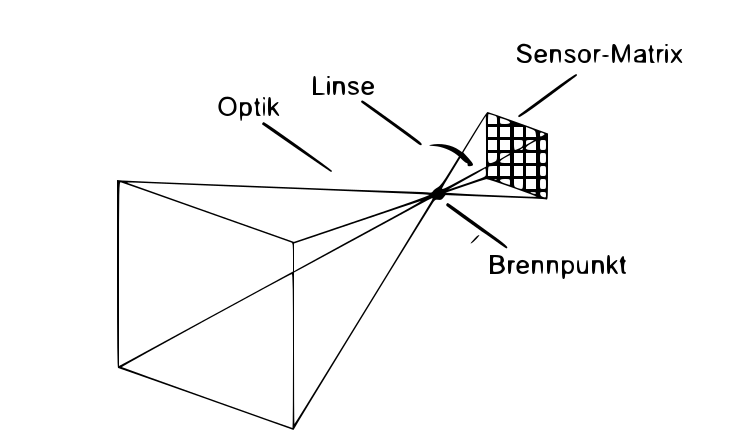
\includegraphics[width=0.8\textwidth]{images/camera_construction.png}
\caption[Digital camera's design]{This image illustrates simply the design of a digital camera, based on Schreer's book \cite{camera_pinhole_model} \label{fig:camera_construction}}
\end{figure}

\begin{figure}
\centering
\includegraphics[width=0.8\textwidth]{images/camera_fov.png}
\caption[Single camera's FoV]{Depicting the influence of the focal length on the field of view, authored by footnote \ref{fov_figure} \label{fig:camera_fov}}
\end{figure}

\subsection{Camera model}\label{camera_model}
In order to illustrate how the transformation from a 3D world coordinate point to a 2D sensor's coordinate system happens, we use the pinhole camera model from Schreer \cite{camera_pinhole_model}. Figure TO\_BE\_ADDED portrays how a point $P$ from a real world object in front of the camera is orthogonally projected on the image plane. We then get the point $C$ definded in the image plane's coordinate system as $(u,v)^{T}$

\subsection{Instance Segmentation Camera}\label{instance_camera}

%###################################################################################
%###################### Topic B             ########################################
%###################################################################################
\section{CARLA - 3D autonomous driving simulator}\label{carla_background}

%###################################################################################
%###################### Topic C             ########################################
%###################################################################################
\section{Related Work}
\chapter{Methodology}
In this chapter we present a detailed problem analysis and discuss our approach for solving the issue.
\label{mainone}
% DELETEME: In this chapter you start addressing your actual problem. Therefore, it makes often sense to make a detailed problem analysis first (if not done in introduction). You should be sure about what to do and how. While writing in the background part, it might also make sense to include complex background information or papers you are basing on in this analysis. If you are solving a software problem, you should follow the state of the art of software development which basically includes: problem analysis, design, implementation, testing, and deployment. Maintenance is often also described but I believe this will not be required for most theses. Code should be placed in the appendix unless it is solving an essential aspect of your work.
\section{Problem Anlaysis}



\section{Approach for Solving the Issue}
This section provides an explanation of what techniques were used in the problem's solution. It is split into smaller subsections, which consider different parts of the proposed strategy.

\subsection{Organisation of the Simulation}
In general, to conduct real-world experiments is rather expensive and time-consuming, therefore we simulate different scenarios using CARLA. What is more, there are no limitations in the digital environment and data samples can be created faster, which contain no distortions or noise. It offers an opportunity to test different approaches and ideas in ideal conditions without any restrictions.

Our simulation takes place in a realistic digital city "Town10HD\_Opt" from the CARLA assets package, which represents a whole town including, i.e., buildings, trees, traffic lights, parked vehicles, etc. The main location of the experiments is a junction of four roads, because, compared to other types of junction, there exists a higher chance for accidents to happen, and an optimal camera placement is crucial for a safe mobility. On the junction's premises we place 3 CARLA objects from type Actor: 
\begin{itemize}
    \item 1 camera and 2 vehicles, which has the roles 'occluder' and 'target'
\end{itemize}
In pursuance of finding an optimal position for the camera sensor we consider the 4 angles of the region of interest (ROI) and also the points in the middle of each of the 4 edges. In this way, we earn an approximate idea which point or area has to be aimed for when placing a camera. Furthermore, this placement could be applied to other infrastructure of the same type, therefore it also guarantees flexibility and universality of the approach. 

With regard to the vehicles, which play the most important role in our research, we divide them into two categories:

\begin{itemize}
    \item \textbf{occluder vehicle} - this is the vehicle that stays between the sensor and the target vehicle and covers some part of it because of its larger size or position regarding the sensor. For a realistic scenario we use a medium and large-sized vans or trucks, so that their shape generate a blind zone for the sensor's field of view, which then cannot recognize the occluded vehicle. 
    \item \textbf{target vehicle} - this vehicle is equal or smaller than the occluder, because we have to measure the degree to which it is occluded in various positions. If, for example, it has the bigger proportions, the chance of a camera not detecting it is quite decreased even if it stays behind the occluder. 
\end{itemize}
During the simulation we spawn both vehicles in different locations on the junction in order to reproduce as many as possible dynamic situations and decide whether an occlusion occurs or not. 

The simulation pipeline consists of three stages:


\chapter{Implementation} \label{implementation}
This chapter describes how the approach we proposed in Chapter \ref{approach} is applied by using the Python API offered by CARLA. Moreover, we reveal the software implementation of the processes behind each of the three stages in our simulation pipeline.  

\section{Setup of Virtual Environment}
The simulation pipeline consists of three main stages - Data Generation for the experiments, Simulation of possible real-world scenarios and Evaluation of the results, as it was explained in the previous chapter. In the course of our first stage, we connect the client to the simulator's server, which represents the digital world for our research. The 3D simulator provides two options for a communication between client and server\footnote{\url{https://carla.readthedocs.io/en/latest/adv_synchrony_timestep/}, visited on 02/12/2022}:
\begin{itemize}
    \item \textbf{synchronous mode} - in this mode the client must notify via tick when all the commands are prepared that the server is obliged to execute. This is the mode which is relevant for simulations where synchrony between, i.e., sensors and world is crucial. 
    \item \textbf{asynchronous mode} - this is the default mode, where the server runs the simulation as fast as possible and does not have to wait for a signal from the client, which ensures that everything is ready for the next step 
\end{itemize}

For this work the synchronous mode is set, because we require an environment, where we know location and rotation of world objects, receive accurate data from the camera and maintain a consistent connection to the server. When we enable the synchronous mode, we create a synchronous instance of the Traffic Manager, which handles any group of vehicles in the simulated world.

\subsection{Sensor placement}
Having all synchrony-related settings adjusted, we then instantiate a new object of type Sensor from CARLA's blueprint library\footnote{\url{https://carla.readthedocs.io/en/latest/bp_library/}, visited on 03/12/2022}. This is a subtype of actor which can measure and stream data. For this thesis the sensor is instance segmentation camera which has the main parameters of each camera sensor: field of view, width and height of generated image. What is more, a sensor is responsible for perceiving data either whenever a new event is registered or on each tick signal received from the client. This sensor in particular has a task to render all elements contained in the field of view with a specific colour according to their semantic tags (vehicle, building, traffic light, etc.) and a unique object ID (assigned by the Unreal Engine at the moment of instantiation). 

With regard to the spawning of sensor, in CARLA one can attach it to a vehicle and thus to visualise an on-board point of view. However, the goal of this thesis is to find an optimal position in the infrastructure, therefore we spawn our traffic monitoring tool as displayed in Figure \ref{fig:camera_positions} on particular locations. Again, there is no algorithm for locations generation, they are completely random and aim to compare three points in each border of the range of interest, which makes eight in total. In order to receive data, which is then forwarded along the pipeline for examination, sensors have an integrated listening method. In short, there we provide as an argument a function that inserts every new image in a queue, which then can be accessed during the evaluation part. At the end, we define the height and tilt angle of the camera so that it points to the intersection and have an unobstructed view.

\subsection{Waypoints generation}
The last step from the first stage is generation of waypoints suitable for our experiments, where pair of vehicles are going to be placed to recreate real-world situations and estimate occlusion percentage, which prevents the camera from a correct perception of the surrounding environment.  
\chapter{Experiments and Evaluation}
\label{evaluation}
% DELETEME: The evaluation chapter is one of the most important chapters of your work. Here, you will prove usability/efficiency of your approach by presenting and interpreting your results. You should discuss your results and interpret them, if possible. Drawing conclusions on the results will be one important point that your estimators will refer to when grading your work.

This chapter serves as a presentation of our the dataset used in our experiments, and their output, after which is discussed if it has met the expectations and the approach was efficient in providing a solution for the camera placement optimisation problem.

\section{Experiments}
In this thesis, two different experiments were conducted in order to evaluate the performance loss of cameras. What is more, with the help of heatmaps and using the metrics M1 and M2 we are able to define an optimal camera position. The experiments aim to check if problems from \ref{problem_analysis} are handled efficiently by the proposed strategy. In the next subsections, we inform about the laptop used for our simulations and explain into details each experiment. Afterwards, we discuss the results and the efficiency of our metrics.

\subsection{Technical specifications}
The following list contains technical specifications of the machine, which all experiments were simulated on:
\begin{itemize}
    \item \textbf{Processor} - Intel Core i7-10750H CPU 2.60GHz
    \item \textbf{RAM} - 16 GB DDR5
    \item \textbf{GPU} - NVIDIA GeForce RTX 3060 6 GB
    \item \textbf{SSD} - 1 TB
\end{itemize}

\newpage
\subsection{First experiment - change height and angle of camera}
The main objective of our first experiment is to evaluate the performance of cameras at different height, because we concluded in Chapter \ref{problem_analysis} that in the found literature there is little information about which height is optimal for traffic surveillance. We use heatmaps to present the highest occlusion degree for each spawn point. Additionally, our metric M2 is applied in order to see what part occlusion situations were from all cases and choose positions which has scored lower values. During the execution of simulations, we rely on a camera with the following configurations:
\begin{itemize}
    \item FoV (horizontal angle) = $80^{\circ}$
    \item Resolution = $1280\times720$ pixels or also known as 720p
\end{itemize}
The reason for our horizontal angle is that we wanted to cover as much as possible from our region of interest and an average traffic surveillance camera on the market has a horizontal field of view $70^{\circ} - 110^{\circ}$. In a real-world scenario, a wider field of view will cause a fisheye effect\footnote{When an image is distorted by stretching the picture around a rounded camera lens} to occur and has to be taken into account. However, in our experiments the conditions are ideal and we do not apply image distortion. We have 8 enumerated positions for the camera, which can be seen in Figure \ref{fig:positions_enumerated}, where we place it at a pre-defined height. On each of these spawn locations for our sensor, we define 6 levels for the height beginning at 5 meters and going to 10 meters with a 1-meter step. This results in 48 simulations, where we set $0^{\circ}$ for the tilt angle at 5 meters, $-10^{\circ}$ at 6 meters and then go to $-30^{\circ}$ at 10 meters with a $-5^{\circ}$ step. In this way we guarantee that the camera has approximately the same sight over the vehicles and the blind spot under the sensor does not increase. The region of interest is limited by the red lines in Figure \ref{fig:positions_enumerated} and is used in each of the two experiments.

During each simulation, we generate a list with waypoints for the target vehicle that are 3 meters apart and one for the occluder, but with 1-meter distance between spawn points. We decided to use Seat Leon (see Fig. \ref{fig:seat_leon}) as a target and Jeep Wrangler Rubicon (see Fig. \ref{fig:jeep_wrangler}) as an occluder for our scenarios, because in an urban area people mainly use normal cars or SUVs for their transportation needs, and therefore it is more often the case that an occlusion-prone situation between these two types of vehicles arises. In our second experiment we consider pairs of vehicles of different type in order to broaden the variety of occlusions.

\begin{figure} [h!]
    \centering
    \includegraphics[width=0.90\textwidth]{images/positions_numerated.png}
    \caption[Enumerated camera positions]{This image shows the number of each camera's position used in our simulations.}
    \label{fig:positions_enumerated}
\end{figure}

\newpage
\subsection{Second experiment - change threshold for target vehicle recognition}
In our second experiment our goal is to observe how strong the occlusion is when there are different types of vehicles. Here we use the same parameters for the camera, but this time it is placed only at 8 meters above the ground. The reason behind this decision is that this value is approximately in the middle between the range of values we used in the previous experiment, and also we have mentioned in Section \ref{main_problems} that the minimum for an ideal height is exactly 8 meters. Furthermore, we guarantee same conditions for all sensor positions by setting their tilt angle at $-20^{\circ}$ in order to have an accurate comparison between each one of them. For this scenario, we use three pairs of vehicles and execute a simulation for each camera position, which comprises a total of 18 simulations, 6 of which are also part of the first experiment. Moreover, we decided to not consider positions 4 and 8 here, because their view is obstructed by the traffic lights and signs on them, therefore their range of view is limited.

For this experiment we rely on the pairs:
\begin{itemize}
    \item Seat Leon and Jeep Wrangler Rubicon
    \item Ford Mustang and Mercedes Sprinter (see Figures \ref{fig:ford_mustang} and \ref{fig:mercedes_sprinter})
    \item Ambulance truck (see Fig. \ref{fig:ambulance}) and Mercedes Sprinter
\end{itemize}
Our idea is to reproduce three possible scenarios in a traffic, in which we have a normal car and SUV, a normal car and a large van, as well as two large-sized vehicles. In this way, we can ensure that a variety of vehicles' sizes are covered by this study. Important to mention is that the distance between target spawn points is again set to 3 meters. 

For the purpose of assessing the optimal camera locations we apply our M1 metric for a priori specified threshold. In the real world it is vital for a camera to miss as little as possible objects, which were hidden due to other large-sized vehicles. Therefore, we set an occlusion tolerance threshold, after which the target vehicle is no more detectable, to 50\%, 75\% and 90\%. By implementing this constraint, we can conclude from the score of our metric how many occlusions from all the detected ones could actually blind the camera. Finally, we choose these positions, which output the lowest values. Apart from the metric, heatmaps display again the maximum occlusion degree for each target position, which was visible for the sensor.


%###################################################################################
%###################### Results             ########################################
%###################################################################################
\section{Results}\label{results}
In the heatmaps and tables below, we can inspect the results from both experiments. In order to maintain a well-arranged visualisation of the output, we are going to present only the heatmaps for 5 and 10-meter height and compare the impact of increasing elevation on the maximum occlusions. For our second experiment, we will visualise the results from cameras placed at 8 meters above the road in positions 1, 3 and 6. The other heatmaps are placed in the appendix, if one wants to analyse them.

\subsection{First experiment} \label{subsec:first_exp_heat}

\begin{figure}[!htb]
\minipage{0.5\textwidth}
  \includesvg[width=\linewidth]{images/position0/pos0_5m.svg}
  \caption{Pos.1 at 5 m height}\label{fig:pos1_5m}
\endminipage\hfill
\minipage{0.5\textwidth}
  \includesvg[width=\linewidth]{images/position0/pos0_10m.svg}
  \caption{Pos.1 at 10 m height}\label{fig:pos1_10m}
\endminipage\hfill
\end{figure}

\newpage
\begin{figure}[!ht]
\minipage{0.5\textwidth}
  \includesvg[width=\linewidth]{images/position1/pos1_5m.svg}
  \caption{Pos.2 at 5 m height}\label{fig:pos2_5m}
\endminipage\hfill
\minipage{0.5\textwidth}
  \includesvg[width=\linewidth]{images/position1/pos1_10m.svg}
  \caption{Pos.2 at 10 m height}\label{fig:pos2_10m}
\endminipage\hfill
\end{figure}

\begin{figure}[!ht]
\minipage{0.5\textwidth}
  \includesvg[width=\linewidth]{images/position2/pos2_5m.svg}
  \caption{Pos.3 at 5 m height}\label{fig:pos3_5m}
\endminipage\hfill
\minipage{0.5\textwidth}
  \includesvg[width=\linewidth]{images/position2/pos2_10m.svg}
  \caption{Pos.3 at 10 m height}\label{fig:pos3_10m}
\endminipage\hfill
\end{figure}

\begin{figure}[!ht]
\minipage{0.5\textwidth}
  \includesvg[width=\linewidth]{images/position3/pos3_5m.svg}
  \caption{Pos.4 at 5 m height}\label{fig:pos4_5m}
\endminipage\hfill
\minipage{0.5\textwidth}
  \includesvg[width=\linewidth]{images/position3/pos3_10m.svg}
  \caption{Pos.4 at 10 m height}\label{fig:pos4_10m}
\endminipage\hfill
\end{figure}

\newpage
\begin{figure}[!ht]
\minipage{0.5\textwidth}
  \includesvg[width=\linewidth]{images/position4/pos4_5m.svg}
  \caption{Pos.5 at 5 m height}\label{fig:pos5_5m}
\endminipage\hfill
\minipage{0.5\textwidth}
  \includesvg[width=\linewidth]{images/position4/pos4_10m.svg}
  \caption{Pos.5 at 10 m height}\label{fig:pos5_10m}
\endminipage\hfill
\end{figure}

\begin{figure}[!ht]
\minipage{0.5\textwidth}
  \includesvg[width=\linewidth]{images/position5/pos5_5m.svg}
  \caption{Pos.6 at 5 m height}\label{fig:pos6_5m}
\endminipage\hfill
\minipage{0.5\textwidth}
  \includesvg[width=\linewidth]{images/position5/pos5_10m.svg}
  \caption{Pos.6 at 10 m height}\label{fig:pos6_10m}
\endminipage\hfill
\end{figure}

\begin{figure}[!ht]
\minipage{0.5\textwidth}
  \includesvg[width=\linewidth]{images/position6/pos6_5m.svg}
  \caption{Pos.7 at 5 m height}\label{fig:pos7_5m}
\endminipage\hfill
\minipage{0.5\textwidth}
  \includesvg[width=\linewidth]{images/position6/pos6_10m.svg}
  \caption{Pos.7 at 10 m height}\label{fig:pos7_10m}
\endminipage\hfill
\end{figure}

\newpage
\begin{figure}[!htb]
\minipage{0.5\textwidth}
  \includesvg[width=\linewidth]{images/position7/pos7_5m.svg}
  \caption{Pos.8 at 5 m height}\label{fig:pos8_5m}
\endminipage\hfill
\minipage{0.5\textwidth}
  \includesvg[width=\linewidth]{images/position7/pos7_10m.svg}
  \caption{Pos.8 at 10 m height}\label{fig:pos8_10m}
\endminipage\hfill
\end{figure}

\begin{table}[!h]
\caption{This table presents the M2 score of each camera position at different height level \label{tab:height_experiment}}
\centering
    \begin{tabular}{ | c | c | c | c | c | c | c | c | c |}
    \hline
    Height & Pos.1 & Pos. 2 & Pos. 3 & Pos. 4 & Pos. 5 & Pos. 6 & Pos. 7 & Pos. 8 \\ \hline
    5 m & 0.50 & 0.49 & 0.70 & 0.52 & 0.54 & 0.55 & 0.74 & 0.68\\ \hline
    6 m & 0.49 & 0.48 & 0.66 & 0.45 & 0.53 & 0.53 & 0.73 & 0.63\\ \hline
    7 m & 0.47 & 0.48 & 0.65 & 0.49 & 0.51 & 0.52 & 0.71 & 0.64\\ \hline
    8 m & 0.48 & 0.47 & 0.63 & 0.48 & 0.51 & 0.50 & 0.68 & 0.61\\ \hline
    9 m & 0.48 & 0.46 & 0.61 & 0.44 & 0.50 & 0.49 & 0.63 & 0.58\\ \hline
    10 m & 0.46 & 0.44 & 0.57 & 0.33 & 0.47 & 0.46 & 0.61 & 0.55\\ \hline
    \end{tabular}
\end{table}

\newpage
\subsection{Second experiment}

\begin{figure}[!htb]
\minipage{0.5\textwidth}
  \includesvg[width=\linewidth]{images/position0/pos0_8m.svg}
  \caption{Pos.1 Seat and Jeep}\label{fig:pos1_8m}
\endminipage\hfill
\minipage{0.5\textwidth}
  \includesvg[width=\linewidth]{images/mustang_sprinter/sprinter_mustang_pos0.svg}
  \caption{Pos.1 Ford and Mercedes}\label{fig:pos1_ford_merc}
\endminipage\hfill
\end{figure}

\newpage
\begin{figure}[!htb]
\minipage{0.5\textwidth}
  \includesvg[width=\linewidth]{images/sprinter_ambulance/ambulance_sprinter_pos0.svg}
  \caption{Pos.1 Ambulance and Mercedes}\label{fig:pos1_amb_merc}
\endminipage\hfill
\minipage{0.5\textwidth}
  \includesvg[width=\linewidth]{images/position2/pos2_8m.svg}
  \caption{Pos.3 Seat and Jeep}\label{fig:pos3_8m}
\endminipage\hfill
\end{figure}

\begin{figure}[!htb]
\minipage{0.5\textwidth}
  \includesvg[width=\linewidth]{images/mustang_sprinter/sprinter_mustang_pos2.svg}
  \caption{Pos.3 Ford and Mercedes}\label{fig:pos3_ford_merc}
\endminipage\hfill
\minipage{0.5\textwidth}
  \includesvg[width=\linewidth]{images/sprinter_ambulance/ambulance_sprinter_pos2.svg}
  \caption{Pos.3 Ambulance and Mercedes}\label{fig:pos3_amb_merc}
\endminipage\hfill
\end{figure}

\begin{figure}[!htb]
\minipage{0.5\textwidth}
  \includesvg[width=\linewidth]{images/position5/pos5_8m.svg}
  \caption{Pos.6 Seat and Jeep}\label{fig:pos6_8m}
\endminipage\hfill
\minipage{0.5\textwidth}
  \includesvg[width=\linewidth]{images/mustang_sprinter/sprinter_mustang_pos5.svg}
  \caption{Pos.6 Ford and Mercedes}\label{fig:pos6_ford_merc}
\endminipage\hfill
\end{figure}

\newpage
\begin{figure}[!htb]
\minipage{0.5\textwidth}
    \includesvg[width=\linewidth]{images/sprinter_ambulance/ambulance_sprinter_pos5.svg}
  \caption{Pos.6 Ambulance and Mercedes}\label{fig:pos6_amb_merc}
\endminipage\hfill
\end{figure}

\begin{table}[!htb]
\caption{This table presents the M1 score at 8 m height for a specified threshold and vehicles Seat Leon and Jeep Wrangler Rubicon\label{tab:jeep_seat_threshold}}
\centering
    \begin{tabular}{ | c | c | c | c | c | c | c |}
    \hline
    Threshold & Pos. 1 & Pos. 2 & Pos. 3 & Pos. 5 & Pos. 6 & Pos. 7 \\ \hline
    50\% & 0.17 & 0.22 & 0.06 & 0.11 & 0.17 & 0.09\\ \hline
    75\% & 0.02 & 0.06 & 0.01 & 0.01 & 0.03 & 0.0\\ \hline
    90\% & 0.0 & 0.0 & 0.01 & 0.0 & 0.0 & 0.0\\ \hline
    \end{tabular}
\end{table}

\newpage
\begin{table}[!htb]
\caption{This table presents the M1 score at 8 m height for a specified threshold and vehicles Ford Mustang and Mercedes Sprinter\label{tab:ford_merc_threshold}}
\centering
    \begin{tabular}{ | c | c | c | c | c | c | c |}
    \hline
    Threshold & Pos. 1 & Pos. 2 & Pos. 3 & Pos. 5 & Pos. 6 & Pos. 7 \\ \hline
    50\% & 0.38 & 0.48 & 0.39 & 0.36 & 0.44 & 0.41\\ \hline
    75\% & 0.24 & 0.31 & 0.21 & 0.18 & 0.26 & 0.22\\ \hline
    90\% & 0.15 & 0.18 & 0.12 & 0.12 & 0.14 & 0.12\\ \hline
    \end{tabular}
\end{table}

\begin{table}[!htb]
\caption{This table presents the M1 score at 8 m height for a specified threshold and vehicles Ambulance Truck and Mercedes Sprinter\label{tab:amb_merc_threshold}}
\centering
    \begin{tabular}{ | c | c | c | c | c | c | c |}
    \hline
    Threshold & Pos. 1 & Pos. 2 & Pos. 3 & Pos. 5 & Pos. 6 & Pos. 7 \\ \hline
    50\% & 0.08 & 0.15 & 0.08 & 0.07 & 0.12 & 0.09\\ \hline
    75\% & 0.0 & 0.0 & 0.0 & 0.0 & 0.0 & 0.0\\ \hline
    90\% & 0.0 & 0.0 & 0.0 & 0.0 & 0.0 & 0.0\\ \hline
    \end{tabular}
\end{table}

%###################################################################################
%###################### Discussions         ########################################
%###################################################################################
\newpage
\section{Discussions}\label{discussions}
In this section we are going to analyse the above displayed heatmaps and tables in order to compare camera's performance in various situations and decide which positions brought the most optimal results. Furthermore, we also discuss which height levels were beneficial the efficiency of our visual sensor.

\subsection{Results of first experiment}
To start with, if we examine the heatmaps from Subsection \ref{subsec:first_exp_heat} and Table \ref{tab:height_experiment}, then we can assert that height is actually of utmost importance for the quantity of detected occlusions. For instance, in Figure \ref{fig:pos1_5m} and Figure \ref{fig:pos1_10m} it is noticeable that the difference of 5 meters significantly decreases the degree of occlusion for each target's spawn location. We are also able to see that our tilt angle is set correctly according to the height and ensures that the same spawn positions remain visible for the camera and new ones also appear at 10 meters. In Figure \ref{fig:pos1_8m} there are still some occlusions higher than 80\%, which still does not achieve the goal we are looking for. 

Out of all positions, there are two offering a lower performance than the other ones - positions 4 and 8. The reason for this behaviour is that there are traffic lights and street signs hanging from the poles, which obstruct their view of the whole region of interest. Moreover, this setback also deprives them of detecting locations on the road, which results in less evaluated situations, as can be asserted from heatmaps \ref{fig:pos4_5m} and \ref{fig:pos8_5m}. However, this outcome proves that our check for points out of the camera's field of view works properly and could also be applied to future experiments for a real-world scenarios.

For this study, it is of interest that an optimal camera position detects fewer occlusions, therefore we used our metric M2 to evaluate which location is efficient for the task. In the table \ref{tab:height_experiment} it makes directly an impression that positions 1 and 2 have scored the lowest values at 5-meter height. However, if we take into account the M2 score of positions 4 and 8, they seem to outperform some other locations, which is not the case. As we mentioned previously, when a sensor is placed there its FoV is limited and sees half the spawn points, which should be in fact recognisable for it. For this reason, their scores will be only valid, if the same amount of target points are available on the image plane. Another important point to be made after examining the table is that with the increase of height, the number of occlusion decreases, which is to be expected due to the fact that the sensor's view angle to the vehicles changes and can monitor them from an unhindered point of view in comparison to the lower heights. At 5, 6 and 7 meters our camera does not show a significant difference in the number of detected occlusions between the test pair of vehicles, whereas over 8 meters the sensor tends to identify with 10-15\% fewer occlusions. With the output of our first experiment, we can consider the statement that an ideal height for a traffic camera starts at 8-meter (see \ref{main_problems}) height as correct.

Finally, after inspecting the heatmaps and the M2 score for each camera placement, positions 1, 2, 3 and 7 guarantee a wider field of view compared to the others, because they have had a larger number of target spawn points in their sight during the experiment. Regarding the quantity of occlusion which is displayed on the heatmap at 10-meter height, position 3 seems to avoid them more efficiently, but its M2 score is the third highest in the table, which means that 57\% of all calculations were occlusions. Nevertheless, this metric is not that accurate when comparing the score at a certain height for different positions, because some positions detect more points around the target vehicle, which allows for more non-occlusion situations and thus the smaller score. In conclusion, we can say that higher placement is crucial, because there are almost no physical view obstructors. Additionally, wider range of view implies better perception of the environment, like it is guaranteed by positions 1, 2, 3 and 7.

\subsection{Results of second experiment}
During this experiment were different types of vehicles involved, which led to a better overview how size of the occluder affects the received quantity of occlusion. For example, when we compare heatmaps \ref{fig:pos1_8m} and \ref{fig:pos1_ford_merc}, it is clear that a camera at the height of 8 meters has a more obstructed view when a Mercedes Sprinter stays in front of a Ford Mustang than in the case when a Jeep Wrangler Rubicon is placed between the sensor and the target vehicle. This ensuing performance we explain by the fact that a Mercedes Sprinter is $2,5-3 m$ tall and for this reason a larger blind zone is formed behind it. Moreover, independent of camera's position this phenomenon occurs in each of the simulations at the height of 8 meters, therefore it is reasonable to place a camera on at a higher level above the road, otherwise the sensor will be less efficient in its tasks.

If we look at Figures \ref{fig:pos6_8m} and \ref{fig:pos6_amb_merc} we notice that there is only a slight difference in the detected occlusion degree, which is due to approximately the same size of the pair of vehicles. What we find surprising in position 6 is that the Mercedes Sprinter has caused less occlusion of the ambulance truck in comparison to the other occluder, but in our opinion the larger size of the trucks is to blame for it. To provide further explanation, more pixels on the image plane represent the ambulance truck as opposed to the Seat Leon, therefore the occlusion degree by the first vehicle increases slower. Nevertheless, if we consider the results from the other heatmaps, it seems that problematic for the sensor are only cases where the occluder vehicle is taller than the target one.

Apart from the heatmaps, we also applied our M1 metric for this experiment in order to investigate what part of all detected occlusions are the ones that exceed a pre-defined threshold. To start with, from Table \ref{tab:jeep_seat_threshold} we realise that in positions 3 and 7 were detected less than 10\% of occlusions, whose degrees were above 50\%. In a real-world situation, 50\% occlusion should not burden an object recognition algorithm, but still to have less severe occlusions monitored is our objective. Subsequently, in the third row the occlusion degrees above 90\% for each position is between 0 and 1\%, which is expected due to the near sizes of both Seat Leon and Jeep Wrangler Rubicon. What is more, it is a rare case that same-sized vehicles cause a full view obstruction to each other, when a camera is placed at least 8 meters above them.

However, if we have a look at Table \ref{tab:ford_merc_threshold}, the values change considerably, as there have been calculated more than 35\% occlusions whose degrees were above 50\%. According to the results, camera positioned at 8 meters is not reliable because it detects numerous occlusions, when we have trucks or vans on the street. Out of all positions 3, 5 and 7 offer a promising performance even in such environmental conditions. On the contrary, positions 2 and 6 tend to suffer more efficiency loss than the other locations, which is due to their rather central position and field of view. As it is illustrated by the heatmaps \ref{fig:pos6_5m} and \ref{fig:pos2_5m}. the number of target spawn points that have been detectable from the camera is low.

Finally, in Table \ref{tab:amb_merc_threshold} we notice that little occlusion occurs between the large-sized vehicles when the threshold is 50\% and above 75\% no occlusion was recorded by the camera, which is an optimal result in case of big vehicles crossing a junction. Taking everything into consideration, positions 3, 5 and 7 have scored the lowest M2 values, which mean they perform well independent of the vehicles' sizes and types.

After having examined and analysed the results of both experiments in detail, we can advance the opinion that positions 3 and 7 outperform the other ones and offer a balance between perceived number of spawn locations and occlusion degree. Definitely, cameras on a higher level (min. 8 m) above the ground have an increased visibility over the road and decrease the blind zone caused by taller vehicles. 

\subsection{Efficiency of metrics}
As we have seen in the previous subsections, two metrics (M1 and M2) were essential for arriving at a decision about which position and which height contribute to an enhanced camera efficiency. Their role in our approach, as described in Section \ref{subsec:metrics}, was to distinguish which occlusions were greater than a pre-defined threshold and to calculate how many out of all examined situations delivered an occlusion. After we have analysed the results, it can be assumed that they fulfilled their task and aided us in determining areas where a camera performs promisingly. However, there were two drawbacks that arose:
\begin{enumerate}
    \item M2 is appropriate, when one investigates the behaviour of camera at a different height on the same position. When the tilt angle is adjusted like in our experiments, a camera can see an identical number of spawn points, because the FoV does not change. If, however, we want to compare positions 3 and 4, we will see in Table \ref{tab:height_experiment} that the second one output lower values, which could lead us to a wrong conclusion about the two positions. Therefore, heatmaps were also involved in the data visualisation, which implied that position 4 has observed 50\% fewer spawn locations and in this way the M2 score gets unreliable. For the purpose of avoiding this issue, it is advisable to extend the metric and compare as well the number of monitored spawn points when studying two positions. Thus, it is ensured that the value of the metric is not influenced by side aspects.
    \item M1 is responsible for evaluating what part of all situations that resulted in occlusion denotes a value which exceeds a threshold for object recognition. Overall, it was accurate and served its role, but does not bring valuable information, as it can be seen at the second two rows in tables \ref{tab:jeep_seat_threshold} and \ref{tab:amb_merc_threshold}, when vehicles of the same size are compared. In our case, cameras were placed at 8 meters above the vehicles, from where it is impossible to have occlusions larger than 80-90\%.
\end{enumerate}

\chapter{Conclusion and Future Work}
\label{conclusion}
%#############################################################
%###################### Summary   ############################
%#############################################################
\section{Summary}
% DELETEME: put a plain summary of your work here. Summaries should be made of each Chapter beginning with Chapter~2 and ending with you evaluation. Just write down what you did and describe the corresponding results without reflecting on them.
At the beginning of this work, we reflect on important scientific information as basis for understanding of the solution we propose. Additionally, we mention various studies in the area of camera placement optimisation, describe their strategies for solving the issue and explain that the ODM of Du et al. in \cite{occlusion_degree_model} serves as inspiration for our approach. Afterwards, in Chapter \ref{problem_analysis} we outline main problems found in the literature during our research. Information about which height should be aimed for and how to decrease occlusion between vehicles are the challenges this thesis was concerned with. In order to investigate which camera positioning is optimal, we present an approach, which includes a 3D simulator as testing environment, two vehicles of equal or different size and an instance segmentation camera. Moreover, the meaning behind our experiments was to see which out of 8 randomly chosen positions is efficient in detecting less occlusions. To provide an insight into our implementation, Chapter \ref{implementation} describes in detail which functionalities of CARLA were used and how our simulation pipeline works, which consists of 3 stages - Data generation, Experiment conduction, Result Evaluation. At the end of the fifth chapter, we discuss our two metrics for comparison of cameras' performance, where the focus is on the number of detected occlusions and those which exceeded a certain threshold (see Section \ref{subsec:metrics}). During the evaluation part, we chose heatmaps and tables to visualise the results, which we then analyse and evaluate. Finally, use the heatmaps and the scores of both metrics to draw a conclusion that positions 3 and 7 outperform the other ones. Some critics for the efficiency of our metrics are provided at the end of Chapter \ref{evaluation}. 

%#############################################################
%###################### Conclusion ###########################
%#############################################################
\section{Conclusion}
% DELETEME: do not summarize here. Reflect on the results that you have achieved. What might be the reasons and meanings of these? Did you make improvements in comparison to the state of the art? What are the good points about your results and work? What are the drawbacks?
Our approach was successful in determining positions for an efficient traffic camera and defining 8 meters as a minimal height. In comparison to studies like \cite{total_coverage_optimum} and \cite{max_camera_coverage} our strategy involves more than one static occlusion, which is examined in a 3D simulator and in this way we provide an enhanced generic approach, which can be applied everywhere. Another benefit of our work is that the impact of height on camera has been tested, which showed that a higher position detects fewer occlusions and have a more accurate view over the road. What is more, in our implementation we used CARLA's instance segmentation camera, which generates ground-truth data and eliminates the necessity of an object detection algorithm. However, if our proposal is to be involved in real-world experiments, depth information should be available and also an algorithm for object recognition must be integrated, because there will be a difference compared to the simulated environment where access to the attributes of each object can be gained. Although our simulations try to approximate dynamic occlusion, they still remain in the area of static experiments. Therefore, if a dynamic scenario has to be represented accurately, the distance between target vehicle spawn locations should be set at least to 0.5 m, which in our experiments is 3 m. What is more, for such shorter distance our algorithm will be slow, especially when large-sized vehicles participate. The reason for this is that we go through 2D arrays of pixels, and therefore either the implementation should be optimised or the constraint for placing occluders, so that only occlusions are perceived by the camera. Nevertheless, our strategy can still provide accurate results for various scenarios, when it is applied in future studies. Some aspects still need to be added, if real-world conditions should be reproduced precisely, which is discussed in the following section.

%#############################################################
%###################### Future Work ##########################
%#############################################################
\section{Future Work}
% DELETEME: Regarding your results - which problems did you not solve? Which questions are still open? Which new questions arose? How should someone / would you continue working in your thesis field basing on your results?

After inspecting the results, we were able to solve the two issues we discussed in the problem analysis. Nevertheless, our approach is focused only on static occlusion and ground truth data, while still lacking some necessary factors for plausible camera performance. For instance, in the future it can be extended by using more vehicles in the simulations in order to observe how traffic density affects object detection and occlusion occurrences. Having mentioned object detection, it is important to implement one of the latest algorithms to see how much time a camera needs to notice a vehicle and combined with our M1 metric it can be realised above what occlusion degree a vehicle is no more visible. By now, we have results for only one camera, therefore further ones can be added to increase the field of view and decrease occlusion by having different points of view. The last suggestion would be to implement some camera constraints as severe weather conditions or image distortion, which will be responsible for reproducing a real-world behaviour.

%__________________________End_of_Thesis______________________________________________
\cleardoublepage
\addcontentsline{toc}{chapter}{Bibliography}
%harvard citations style, please uncomment harvard package in the usepackage area
%\bibliographystyle{agsm}
%remove the following line when using harvard style citation
%\bibliographystyle{plainnat}
\bibliographystyle{unsrt}
%specify bibtex file here
\bibliography{input/mybib}
%add appendix to TOC
\addcontentsline{toc}{chapter}{Appendices}
\chapter*{Appendices}
\label{appendices}
%###################################################################################
%###################### Appendix A          ########################################
%###################################################################################
%\newpage
\addcontentsline{toc}{section}{Appendix A: Abbreviations}
\section*{Appendix A: Abbreviations}
\begin{center}
\begin{tabular}{ll}
\textbf{FoV}	&	Field of View\\
\textbf{LiDAR}	&	Light Detection and Ranging\\
\textbf{ODM}	&	Occlusion Degree Model (mathematical model)\\
\textbf{RGBA}	&	Red, Green, Blue and Alpha (opacity index)\\
\textbf{ROI}	&	Region of Interest\\
\textbf{CPO}	&	Camera Placement Optimisation\\
%\textbf{abk}	&	erklärung\\
%\textbf{abk}	&	erklärung\\
%\textbf{abk}	&	erklärung\\
%\textbf{abk}	&	erklärung\\
%\textbf{abk}	&	erklärung\\
%\textbf{abk}	&	erklärung\\
%\textbf{abk}	&	erklärung\\
%\textbf{abk}	&	erklärung\\
\end{tabular}
\end{center}

%###################################################################################
%###################### Appendix B          ########################################
%###################################################################################
\newpage
\addcontentsline{toc}{section}{Appendix B: Link to GitLab repository}
\section*{Appendix B: GitLab Link}

Here is the link to my GitLab repository, where the Python scripts used for implementation of our approach are available in folder \textit{camera\_optimization}: \url{https://git.tu-berlin.de/georgik1609/bachelor_thesis}, visited on 21/12/2022.

\newpage
\addcontentsline{toc}{section}{Appendix C: Images of town and vehicles}
\section*{Appendix C: Images of town and vehicles}
In this section we present pictures of the town and vehicles with their bounding boxes to get a visual idea of the environment and its actors that participated in our simulations. The lightbulbs and projectors are shown because images were made in editor mode, but have nothing to do with the thesis.
\begin{figure} [h!]
    \centering
    \includegraphics[width=\textwidth]{images/experiment_city.png}
    \caption[Environment for experiments]{This picture shows how the city which we used for our simulations is designed. In the middle, the junction can be seen.}
    \label{fig:city_experiments}
\end{figure}

\newpage
\begin{figure} [h!]
    \centering
    \includegraphics[width=0.5\textwidth]{images/mercedes_sprinter.png}
    \caption[Mercedes Sprinter]{Mercedes Sprinter}
    \label{fig:mercedes_sprinter}
\end{figure}

\begin{figure} [h!]
    \centering
    \includegraphics[width=0.5\textwidth]{images/seat_leon.png}
    \caption[Seat Leon]{Seat Leon}
    \label{fig:seat_leon}
\end{figure}

\begin{figure} [h!]
    \centering
    \includegraphics[width=0.5\textwidth]{images/ambulance.png}
    \caption[Ambulance]{Ambulance}
    \label{fig:ambulance}
\end{figure}

\begin{figure} [h!]
    \centering
    \includegraphics[width=0.5\textwidth]{images/jeep_wrangler_rubicon.png}
    \caption[Jeep Wrangler Rubicon]{Jeep Wrangler Rubicon}
    \label{fig:jeep_wrangler}
\end{figure}

\begin{figure} [h!]
    \centering
    \includegraphics[width=0.5\textwidth]{images/ford_mustang.png}
    \caption[Ford Mustang]{Ford Mustang}
    \label{fig:ford_mustang}
\end{figure}

\newpage
\addcontentsline{toc}{section}{Appendix D: Heatmaps from experiments}
\section*{Appendix D: Heatmaps from experiments} \label{appendix_heatmaps}

Here we display the rest of our heatmaps, which can be used to get a clear idea of the camera's performance in each executed simulation. To clarify, from Figure \ref{fig:pos2_8m} on, all the heatmaps represent the results from the second experiment for a camera placed at 8-meter height.

\begin{figure}[!htb]
\minipage{0.5\textwidth}
  \includesvg[width=\linewidth]{images/position0/pos0_6m.svg}
  \caption{Pos.1 at 6 m height}\label{fig:pos1_6m}
\endminipage\hfill
\minipage{0.5\textwidth}
  \includesvg[width=\linewidth]{images/position0/pos0_7m.svg}
  \caption{Pos.1 at 7 m height}\label{fig:pos1_7m}
\endminipage\hfill
\end{figure}

\begin{figure}[!htb]
\minipage{0.5\textwidth}
  \includesvg[width=\linewidth]{images/position0/pos0_9m.svg}
  \caption{Pos.1 at 9 m height}\label{fig:pos1_9m}
\endminipage\hfill
\minipage{0.5\textwidth}
  \includesvg[width=\linewidth]{images/position1/pos1_6m.svg}
  \caption{Pos.2 at 6 m height}\label{fig:pos2_6m}
\endminipage\hfill
\end{figure}

\begin{figure}[!htb]
\minipage{0.5\textwidth}
  \includesvg[width=\linewidth]{images/position1/pos1_7m.svg}
  \caption{Pos.2 at 7 m height}\label{fig:pos2_7m}
\endminipage\hfill
\minipage{0.5\textwidth}
  \includesvg[width=\linewidth]{images/position1/pos1_9m.svg}
  \caption{Pos.2 at 9 m height}\label{fig:pos2_9m}
\endminipage\hfill
\end{figure}

\begin{figure}[!htb]
\minipage{0.5\textwidth}
  \includesvg[width=\linewidth]{images/position2/pos2_6m.svg}
  \caption{Pos.3 at 6 m height}\label{fig:pos3_6m}
\endminipage\hfill
\minipage{0.5\textwidth}
  \includesvg[width=\linewidth]{images/position2/pos2_7m.svg}
  \caption{Pos.3 at 7 m height}\label{fig:pos3_7m}
\endminipage\hfill
\end{figure}

\begin{figure}[!htb]
\minipage{0.5\textwidth}
  \includesvg[width=\linewidth]{images/position2/pos2_9m.svg}
  \caption{Pos.3 at 9 m height}\label{fig:pos3_9m}
\endminipage\hfill
\minipage{0.5\textwidth}
  \includesvg[width=\linewidth]{images/position3/pos3_6m.svg}
  \caption{Pos.4 at 6 m height}\label{fig:pos4_6m}
\endminipage\hfill
\end{figure}

\begin{figure}[!htb]
\minipage{0.5\textwidth}
  \includesvg[width=\linewidth]{images/position3/pos3_7m.svg}
  \caption{Pos.4 at 7 m height}\label{fig:pos4_7m}
\endminipage\hfill
\minipage{0.5\textwidth}
  \includesvg[width=\linewidth]{images/position3/pos3_9m.svg}
  \caption{Pos.4 at 9 m height}\label{fig:pos4_9m}
\endminipage\hfill
\end{figure}

\begin{figure}[!htb]
\minipage{0.5\textwidth}
  \includesvg[width=\linewidth]{images/position4/pos4_6m.svg}
  \caption{Pos.5 at 6 m height}\label{fig:pos5_6m}
\endminipage\hfill
\minipage{0.5\textwidth}
  \includesvg[width=\linewidth]{images/position4/pos4_7m.svg}
  \caption{Pos.5 at 7 m height}\label{fig:pos5_7m}
\endminipage\hfill
\end{figure}

\begin{figure}[!htb]
\minipage{0.5\textwidth}
  \includesvg[width=\linewidth]{images/position4/pos4_9m.svg}
  \caption{Pos.5 at 9 m height}\label{fig:pos5_9m}
\endminipage\hfill
\minipage{0.5\textwidth}
  \includesvg[width=\linewidth]{images/position5/pos5_6m.svg}
  \caption{Pos.6 at 6 m height}\label{fig:pos6_6m}
\endminipage\hfill
\end{figure}

\begin{figure}[!htb]
\minipage{0.5\textwidth}
  \includesvg[width=\linewidth]{images/position5/pos5_7m.svg}
  \caption{Pos.6 at 7 m height}\label{fig:pos6_7m}
\endminipage\hfill
\minipage{0.5\textwidth}
  \includesvg[width=\linewidth]{images/position5/pos5_9m.svg}
  \caption{Pos.6 at 9 m height}\label{fig:pos6_9m}
\endminipage\hfill
\end{figure}

\begin{figure}[!htb]
\minipage{0.5\textwidth}
  \includesvg[width=\linewidth]{images/position6/pos6_6m.svg}
  \caption{Pos.7 at 6 m height}\label{fig:pos7_6m}
\endminipage\hfill
\minipage{0.5\textwidth}
  \includesvg[width=\linewidth]{images/position6/pos6_7m.svg}
  \caption{Pos.7 at 7 m height}\label{fig:pos7_7m}
\endminipage\hfill
\end{figure}

\begin{figure}[!htb]
\minipage{0.5\textwidth}
  \includesvg[width=\linewidth]{images/position6/pos6_9m.svg}
  \caption{Pos.7 at 9 m height}\label{fig:pos7_9m}
\endminipage\hfill
\minipage{0.5\textwidth}
  \includesvg[width=\linewidth]{images/position7/pos7_6m.svg}
  \caption{Pos.8 at 6 m height}\label{fig:pos8_6m}
\endminipage\hfill
\end{figure}

\begin{figure}[!htb]
\minipage{0.5\textwidth}
  \includesvg[width=\linewidth]{images/position7/pos7_7m.svg}
  \caption{Pos.8 at 7 m height}\label{fig:pos8_7m}
\endminipage\hfill
\minipage{0.5\textwidth}
  \includesvg[width=\linewidth]{images/position7/pos7_9m.svg}
  \caption{Pos.8 at 9 m height}\label{fig:pos8_9m}
\endminipage\hfill
\end{figure}

\begin{figure}[!htb]
\minipage{0.5\textwidth}
  \includesvg[width=\linewidth]{images/position1/pos1_8m.svg}
  \caption{Pos.2 Seat and Jeep}\label{fig:pos2_8m}
\endminipage\hfill
\minipage{0.5\textwidth}
  \includesvg[width=\linewidth]{images/mustang_sprinter/sprinter_mustang_pos1.svg}
  \caption{Pos.2 Ford and Mercedes}\label{fig:pos2_ford_merc}
\endminipage\hfill
\end{figure}

\newpage
\begin{figure}[!htb]
\minipage{0.5\textwidth}
  \includesvg[width=\linewidth]{images/sprinter_ambulance/ambulance_sprinter_pos1.svg}
  \caption{Pos.2 Ambulance and Mercedes}\label{fig:pos2_amb_merc}
\endminipage\hfill
\minipage{0.5\textwidth}
  \includesvg[width=\linewidth]{images/position4/pos4_8m.svg}
  \caption{Pos.5 Seat and Jeep}\label{fig:pos5_8m}
\endminipage\hfill
\end{figure}

\begin{figure}[!htb]
\minipage{0.5\textwidth}
  \includesvg[width=\linewidth]{images/mustang_sprinter/sprinter_mustang_pos4.svg}
  \caption{Pos.5 Ford and Mercedes}\label{fig:pos5_ford_merc}
\endminipage\hfill
\minipage{0.5\textwidth}
  \includesvg[width=\linewidth]{images/sprinter_ambulance/ambulance_sprinter_pos4.svg}
  \caption{Pos.5 Ambulance and Mercedes}\label{fig:pos5_amb_merc}
\endminipage\hfill
\end{figure}

\begin{figure}[!htb]
\minipage{0.5\textwidth}
  \includesvg[width=\linewidth]{images/position6/pos6_8m.svg}
  \caption{Pos.7 Seat and Jeep}\label{fig:pos7_8m}
\endminipage\hfill
\minipage{0.5\textwidth}
  \includesvg[width=\linewidth]{images/mustang_sprinter/sprinter_mustang_pos6.svg}
  \caption{Pos.7 Ford and Mercedes}\label{fig:pos7_ford_merc}
\endminipage\hfill
\end{figure}

\newpage
\begin{figure}[!htb]
\minipage{0.5\textwidth}
    \includesvg[width=\linewidth]{images/sprinter_ambulance/ambulance_sprinter_pos6.svg}
  \caption{Pos.7 Ambulance and Mercedes}\label{fig:pos7_amb_merc}
\endminipage\hfill
\end{figure}

% \newpage
% %change this
% \addcontentsline{toc}{section}{Appendix C: {\LaTeX} Help}
% \section*{Appendix C: {\LaTeX} Help}
% %remove this
% \input{help/latex_hinweise}



\end{document}
